\documentclass[12pt]{article}

\usepackage{answers}
\usepackage{setspace}
\usepackage{graphicx}
\usepackage{enumitem}
\usepackage{multicol}
\usepackage{mathrsfs}
\usepackage[margin=1in]{geometry} 
\usepackage{amsmath,amsthm,amssymb}
\usepackage[english]{babel}

\newcommand{\N}{\mathbb{N}}
\newcommand{\Z}{\mathbb{Z}}
\newcommand{\C}{\mathbb{C}}
\newcommand{\R}{\mathbb{R}}

\DeclareMathOperator{\sech}{sech}
\DeclareMathOperator{\csch}{csch}

\newenvironment{theorem}[2][Theorem]{\begin{trivlist}
		\item[\hskip \labelsep {\bfseries #1}\hskip \labelsep {\bfseries #2.}]}{\end{trivlist}}
\newenvironment{definition}[2][Definition]{\begin{trivlist}
		\item[\hskip \labelsep {\bfseries #1}\hskip \labelsep {\bfseries #2.}]}{\end{trivlist}}
\newenvironment{proposition}[2][Proposition]{\begin{trivlist}
		\item[\hskip \labelsep {\bfseries #1}\hskip \labelsep {\bfseries #2.}]}{\end{trivlist}}
\newenvironment{lemma}[2][Lemma]{\begin{trivlist}
		\item[\hskip \labelsep {\bfseries #1}\hskip \labelsep {\bfseries #2.}]}{\end{trivlist}}
\newenvironment{exercise}[2][Exercise]{\begin{trivlist}
		\item[\hskip \labelsep {\bfseries #1}\hskip \labelsep {\bfseries #2.}]}{\end{trivlist}}
\newenvironment{solution}[2][Solution]{\begin{trivlist}
		\item[\hskip \labelsep {\bfseries #1}]}{\end{trivlist}}
\newenvironment{problem}[2][Problem]{\begin{trivlist}
		\item[\hskip \labelsep {\bfseries #1}\hskip \labelsep {\bfseries #2.}]}{\end{trivlist}}
\newenvironment{question}[2][Question]{\begin{trivlist}
		\item[\hskip \labelsep {\bfseries #1}\hskip \labelsep {\bfseries #2.}]}{\end{trivlist}}
\newenvironment{corollary}[2][Corollary]{\begin{trivlist}
		\item[\hskip \labelsep {\bfseries #1}\hskip \labelsep {\bfseries #2.}]}{\end{trivlist}}

\begin{document}
	\title{Robotics 1 - Summary}
	\author{Michael Gabler}
	\maketitle
	\tableofcontents
	\newpage
	
	\section{Basics}
	\subsection{Definitions}
	\textbf{Degrees of freedom}: Defines how many axes of the robot can be manipulated\\
	\textbf{Joints (Gelenke)}: The robot's joints can be \textbf{r}evolute (rotating) or \textbf{p}rismatic (expanding)\\
	\textbf{Joint variable}: The value that describes the state of the joint. This is the current length for prisamtic joints and the rotation angle for revolute joints.\\
	\textbf{Work envelope}: All points that can be reaced with the endeffector\\
	\textbf{Coordinate frames}: $[v]^M$ points out that the values of vector $v$ are in the coordinate frame $M$.
	
	\subsection{Mathematical Background}
	\paragraph{Sinus, Cosinus, Tangenz}
	Short formes: $S_{k} = \sin \theta_{k}$, $C_{k} = \cos \theta_{k}$\\
	$\arctan(\frac{y}{x}) \in ]-\frac{\pi}{2};\frac{\pi}{2}[$: to find all solutions use the $\arctan2$ instead:
	\begin{equation}
	\arctan2(y,x) = 
	\left\{ \begin{array}{ll}
	\arctan(\frac{y}{x}), & x > 0\\
	sgn(y)\frac{\pi}{2}, & x = 0\\
	\arctan(\frac{y}{x}) + sgn(y)\pi, & x < 0, y \neq 0\\
	\pi, & x < 0, y = 0
	\end{array} \right.
	\end{equation}
	
	\paragraph{Matrices and vectors}
	$I$: Identiymatrix, 0 for every element exept the diagonal from top left to bottom right\\
	Inverse matrix $M^{-1}$: $M^{-1} M = I$
	
	\subsubsection{Transformations}
	Describe how a coordinate frame is located in respect to a base reference frame.
	\paragraph{Fundamental rotation matrices} $R_{n}(\phi)$ describes the rotation around the n axe with the angle $\phi$.\\
	\begin{equation}
	R_{1}(\phi) = 
	\begin{bmatrix}
	1 & 0 & 0\\
	0 & \cos \phi & -\sin \phi\\
	0 & \sin \phi & \cos \phi
	\end{bmatrix}
	\end{equation}
	\begin{equation}
	R_{2}(\phi) = 
	\begin{bmatrix}
	\cos \phi & 0 & \sin \phi\\
	0 & 1 & 0\\
	-\sin \phi & 0 & \cos \phi
	\end{bmatrix}
	\end{equation}
	\begin{equation}
	R_{3}(\phi) = 
	\begin{bmatrix}
	\cos \phi & -\sin \phi & 0\\
	\sin \phi & \cos \phi & 0\\
	0 & 0 & 1
	\end{bmatrix}
	\end{equation}
	
	\paragraph{Yaw-Pitch-Roll transformation} Rotate around $f^1$ with $\theta_{1}$, $f^2$ with $\theta_{2}$ and $f^3$ with $\theta_{3}$
	\begin{equation}
	YPR(\theta) = 
	\begin{bmatrix}
	C_{2} C_{3} & S_{1} S_{2} C_{3} - C_{1} S_{3} & C_{1} S_{2} C_{3} + S_{1} S_{3}\\
	C_{2} S_{3}  & S_{1} S_{2} S_{3} + C_{1} C_{3} & C_{1} S_{2} S_{3} - S_{1} C_{3}\\
	-S_{2} & S_{1} C_{2} & C_{1} C_{2}
	\end{bmatrix}
	\end{equation}
	
	\paragraph{Euler Angles transformation} Rotate around $m^3$ with $\theta_{1}$, $m^2$ with $\theta_{2}$ and $m^3$ with $\theta_{3}$ again
	\begin{equation}
	R_{3}(\theta_{1}) R_{2}(\theta_{2}) R_{3}(\theta_{3}) = 
	\begin{bmatrix}
	C_{1} C_{2} C_{3} - S_{1} S_{3} & -C_{1} C_{2} S_{3} - S_{1} C_{3} & C_{1} S_{2}\\
	S_{1} C_{2} C_{3} + C_{1} S_{3}  & -S_{1} C_{2} S_{3} + C_{1} C_{3} & S_{1} S_{2}\\
	-S_{2} C_{3} & S_{2} S_{3} & C_{2}
	\end{bmatrix}
	\end{equation}
	
	\paragraph{Homogenous transformation} Describe coordinates as homogenous coordinates to describe rotations and translations\\
	vector $q$ as homogenous coordinates is $[q_{1} q_{2} q_{3} 1]^T$\\
	Homogenous transformation matrix
	\begin{equation}
	T = 
	\begin{bmatrix}
	R & p\\
	\eta^T & \sigma
	\end{bmatrix}
	\end{equation}
	with\\
	$R \in \mathbf{R}^{3 \times 3}$ is a rotation matrix\\
	$p \in \mathbf{R}^{3 \times 1}$ is a translation vector\\
	$\sigma \in \mathbf{R}$ is a scaling factor (usually 1)\\
	$\eta^T \in \mathbf{R}^{1 \times 3}$ is a perspective vector, here zero vector	\begin{equation}
	Rot(\phi, k) = 
	\begin{bmatrix}
	& & & 0\\
	& R_{k}(\phi) & & 0\\
	& & & 0\\
	0 & 0 & 0 & 1
	\end{bmatrix}, 
	Tran(p) = 
	\begin{bmatrix}
	1 & 0 & 0 & p_{1}\\
	0 & 1 & 0 & p_{2}\\
	0 & 0 & 1 & p_{3}\\
	0 & 0 & 0 & 1
	\end{bmatrix}
	\end{equation}
	
	Calculate arbitrary transformations by using the following rules:
	\begin{enumerate}
		\item Start with $T = I$, $F$ (fixed frame) and $M$ (mobile frame) are equivalent
		\item Represent rotations and translations as separate fundamental homogenous transformation matrices
		\item If $M$ is rotated about or translated along a unit vector of $F$, \textbf{premultiply} homogenous transformation matrix to $T$
		\item If $M$ is rotated about or translated along a unit vector of $M$, \textbf{postmultiply} homogenous transformation matrix to $T$
	\end{enumerate}

	% TODO: how to transform coodinates from one frame to another?
	
	\paragraph{Inverse homogenous transformation} If the transformation matrix $T$ maps coordinates from coordinate frame $A$ to $B$, the inverse $T^{-1}$ maps coodinates from $B$ to $A$.
	\begin{equation}
	T^{-1} = 
	\begin{bmatrix}
	& R^T & & -R^T p\\
	0 & 0 & 0 & 1
	\end{bmatrix}
	\end{equation}
	with $\eta = 0$ and $\sigma = 1$
	
	\paragraph{Screw transformation} rotation of $\phi$ and translation of $\lambda$ around/about the same axis $k$ (unit vector of $F$) like the movement with a screw driver
	\begin{equation}
	Screw(\lambda,\phi,k) = Rot(\phi , k) Tran(\lambda i^k)
	\end{equation}
	with $i^k$ as $k$-th unit vector
	
	\section{Manipulators}
	\subsection{Direct kinematics}
	Direct kinematics is the determination of the tool tip's coordinates and orientation in the base coordinate frame when the values for the joint variables are given.
	\subsubsection{Right-Hand Rules}
	The assignment of the axis of a coodinate frame follows the right-hand rule (see figure \ref{fig:right-hand-frame}).\\
	\begin{figure}[h]
		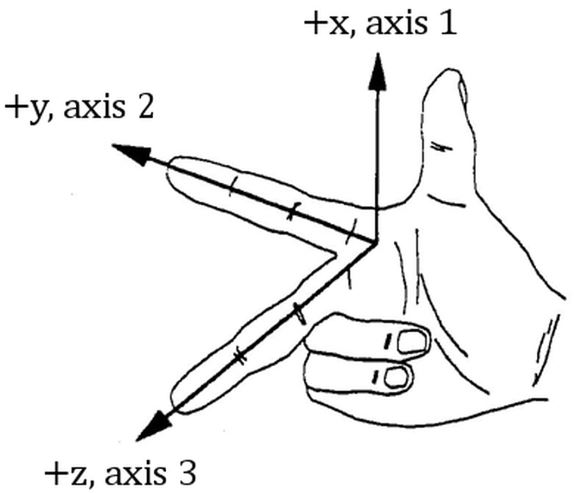
\includegraphics[width=0.5\textwidth]{figures/right-hand-frame.JPG}
		\caption{Right-handed coordinate frame}
		\label{fig:right-hand-frame}
	\end{figure}
	To determine the positive direction of a rotation angle use the right-hand rule by pointing the thumb in the positive direction of the rotation axis. The remaining fingers indicate the positive direction of rotation. (see figure \ref{fig:right-hand-rule})
	\begin{figure}[h]
		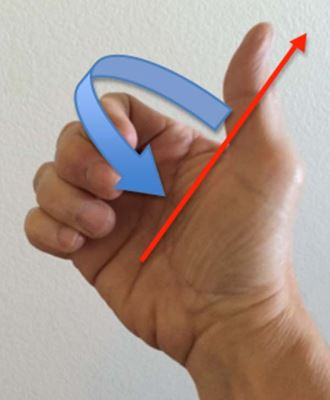
\includegraphics[width=0.5\textwidth]{figures/right-hand-rule.JPG}
		\caption{Right-hand rule}
		\label{fig:right-hand-rule}
	\end{figure}
	
	\subsubsection{Kinematic parameters}
	Specify the kinematic configuration of a robot. There are $4n$ parameters for a $n$-axis robot, 4 for each link/joint, one of them is variable and is called \textbf{joint variable}.
	
	\begin{tabular}{|l|c|c|c|}
		\hline
		\textbf{Arm parameter} & \textbf{Symbol} & \textbf{Revolute joint} & \textbf{Prismatic joint} \\ \hline
		Joint angle            &    $\theta$     &        variable         &          fixed           \\ \hline
		Joint distance         &       $d$       &          fixed          &         variable         \\ \hline
		Link length            &       $a$       &          fixed          &          fixed           \\ \hline
		Link twist angle       &    $\alpha$     &          fixed          &          fixed           \\ \hline
	\end{tabular} 
	
	\subsubsection{Denavit-Hartenberg Algorithm}
	The Denavit-Hartenberg Algorithm is used to assign coordinate frames to each link of the robot and to determine the kinematic parameters of the robot.\\
	Numbering of links: $0$ (fixed base) to $n$ at the tool $\Rightarrow$ $n+1$ links for $n$-axis robot\\
	Numbering of joints: joint $k$ interconnects link $k-1$ with link $k$ with $1 \leq k \leq n$
	\paragraph{Part 1: Assignment of coordinate frames}
	\begin{enumerate}
		\item Number the joints from $1$ to $n$
		\item Assign a right-handed orthonormal coordinate frame $L_0$ to robot base, making sure that $z^0$ aligns with the axis of joint $1$. Set $k = 1$.
		\item Align $z^k$ with the axis of joint $k + 1$.
		\item Locate the orign of $L_k$ at the intersection of the $z^k$ and $z^{k-1}$ axes.\\
		If they are not parallel and do not intersect, use the intersection of $z^k$ with a common normal between $z^k$ and $z^{k-1}$.\\
		If they are parallel, use the intersection of $z^k$ with either a normal between $z^k$ and $z^{k+1}$ or the normal between $z^k$ and $z^{k-1}$ intersecting the origin of $L_{k-1}$.
		\item Select $x^k$ to be orthogonal to both $z^k$ and $z^{k-1}$, making sure that $x^k$ intersects $z^{k-1}$. $x^k$ should point away from $z^{k-1}$.
		\item Select $y^k$ to form a right-handed orthonormal coordinate frame $L_k$.
		\item Set $k \leftarrow k + 1$. If $k < n$, go to step 3, else continue.
		\item Set the origin of $L_n$ at the tool tip. Align $z^n$ with the approach vector, $y^n$ with the sliding vector and $x^n$ with the normal vector of the tool.\\
		Set $k = 1$ and continue with part 2.
	\end{enumerate}
	\paragraph{Part 2: Determination of kinematic parameters}
	\begin{enumerate}
		\item Locate point $b_k$ at the intersection of the $x^k$ and $z^{k-1}$ axes.\\
		Only in case $k = n$: If they do not intersect, use the intersection of $x^k$ with a common normal between $x^k$ and $z^{k-1}$
		\item Compute $\theta_{k}$ as the angle of rotation from $x^{k-1}$ to $x^k$ measured about $z^{k-1}$.
		\item Compute $d_k$ as the distance from the origin of frame $L_{k-1}$ to point $b_k$ measured along $z^{k-1}$.
		\item Compute $a_k$ as the distance from point $b_k$ to the origin of frame $L_k$ measured along $x^k$.
		\item Compute $\alpha_k$ as the angle of rotation from $z^{k-1}$ to $z^k$ measured about $x^k$.
		\item Set $k \leftarrow k + 1$. If $k \leq n$, go to step 1, else stop.
	\end{enumerate}
	
	\subsubsection{Arm equation}
	The arm equation defines a transformation matrix $T^{tool}_{base}(q)$ that transforms coordinates of the tool coordinate frame $L_n$ to the base coordinate frame $L_0$ and depends on the vector of joint variables $q$ (see equation \ref{eq:transform-tool-base}). It is composed out of several transformations between the link coodinate frames (see equation \ref{eq:transform-lcf}).
	\begin{equation}
	T^{k}_{k-1} = 
	\begin{bmatrix}
	C \theta_k & -C \alpha_k S \theta_k & S \alpha_k S \theta_k & a_k C \theta_k\\
	S \theta_k & C \alpha_k C \theta_k & -S \alpha_k C \theta_k & a_k S \theta_k\\
	0 & S \alpha_k & C \alpha_k & d_k\\
	0 & 0 & 0 & 1
	\end{bmatrix}
	\label{eq:transform-lcf}
	\end{equation}
	\begin{equation}
	(T^{k}_{k-1})^{-1} = T^{k-1}_{k} = 
	\begin{bmatrix}
	C \theta_k & S \theta_k & 0 & -a_k\\
	-C \alpha_k S \theta_k & C \alpha_k C \theta_k & S \alpha_k & -d_k S \alpha_k\\
	S \alpha_k S \theta_k & -S \alpha_k C \theta_k & C \alpha_k & -d_k C \alpha_k\\
	0 & 0 & 0 & 1
	\end{bmatrix}
	\end{equation}
	\begin{equation}
	T^{tool}_{base}(q) = T^1_0(q_1) T^2_1(q_2) ... T^n_{n-1}(q_n) = 
	\begin{bmatrix}
	& R(q) & & p(q)\\
	0 & 0 & 0 & 1
	\end{bmatrix}
	\label{eq:transform-tool-base}
	\end{equation}
	$R(q) \in \mathbf{R}^{3 \times 3}$ the orientation of the tool as rotation matrix.\\
	The three columns of $R(q)$ are the three unit vectors of the tool frame in relation to the base frame.\\
	\\
	$p(q) \in \mathbf{R}^3$ the translation vector and therefore the position of the tool tip in relation to the base frame.
	
	\subsection{Inverse kinematics}
	Inverse kinematics describes the task to determine the robot's joint variables when the tool tip's coordinates and orientation (called the tool configuration) is given. There are often multiple solutions because the position can be reached by different alignment of the joints.
	
	\subsubsection{Tool-configuration space}
	To describe the tool tip's coordinates and orientation one can use a $\mathbf{R}^6$-vector which is called the tool-configuration vector $w$.\\
	\begin{equation}
	w = 
	\begin{bmatrix}
	w_1 \\ w_2 \\ w_3 \\ w_4 \\ w_5 \\ w_6
	\end{bmatrix} = 
	\begin{bmatrix}
	p \\ e^{\frac{q_n}{\pi}}r^3
	\end{bmatrix}
	\end{equation}
	with $p \in \mathbf{R}^3$ the translation vector of the arm equation's vector $T^{tool}_{base}$\\
	$q \in \mathbf{R}^n$ the vector of joint variables for a robot with $n$-joints\\
	$r^3 \in \mathbf{R}^3$ the third column vector of the rotation matrix $R$ from $T^{tool}_{base}$
	
	\subsubsection{Solving the inverse kinematic}
	Construct a vector $w$ by calculating the matrix $T^{tool}_{base}$ and taking the equations from there. $w_1, ..., w_6$ is given, so it's possible to solve the equation system for all values of the joint variables vector $q$.\\
	\textbf{Hint}: $q_n = \pi \ln \sqrt{w_4^2+w_5^2+w_6^2}$

	\subsubsection{Work space}
	\textbf{Joint-space work envelope} describes all values that are possible for the joint variables. They have to be between $q^{min}$ and $q^{max}$ which denote the minimal and maximal limits of the joints.\\
	\textbf{Work envelope} describes all points $p$ that are reachable with the tool tip. This results from the joint-space work envelope.
	
	\subsubsection{Trajectory planning}
	The trajectory describes a path on which the tool tip moves to get from one point to another and at what time the tool tip has to be located at which point in between.\\
	\textbf{Speed distribution function} $s(t) = \lambda$ maps every $t \in [0;T]$ to the values $\lambda \in [0;1]$. $t$ describes the current time on the path where $T$ is the time at which the target point is reached. $s(0) = 0$ and $s(T) = 1$.\\
	\textbf{Speed profile} $\dot{s}(t)$ is the derivative of the speed distribution function and puts out the velocity for each $t$.\\
	\textbf{Acceleration} The current acceleration is given by the derivative of the speed profile $\ddot{s}(t)$.\\
	\textbf{Straight line motion} connects to points on the shortest possible way. To calculate the current tool-configuration vector use: $w(t) = (1-s(t))w^0 + s(t)w^1$ with $w^0$ as initial and $w^1$ as target position.\\
	\textbf{Joint velocity} $\dot{q}_k$ can be calculated by deriving the equations for the inverse kinematic. This value is directly proportional to the output speed of the $k$-th joint motor.\\
	\textbf{Problems of trajectory planning}
	\begin{itemize}
		\item Singularities: points in work envelope where a total different orientation of the joints is required to reach the next point (would require infinite acceleration)
		\item Path of knot points: for continuous motion infinite accelerations would be applied (instead stop at every knot point and do separate trajectory plannings) $\rightarrow$ at least two continuous derivatives of $w(t)$ required
	\end{itemize}

	\paragraph{Cubic Polynomial Interpolation} Define a trajectory with this function: $w(t) = at^3 + bt^2 + ct + d$ for $0 \leq t \leq T$ which can be derivated two times. Solve with the following constraints:\\
	$w(0) = w^0$, $w(T) = w^1$, $v(0) = \dot{w}(0) = v^0$, $v(T) = \dot{w}(T) = v^1$\\
	For trajectory through more than two points, use higher-degree interpolating polynomial, choose velocities for the points and construct the new constraint equations
	
	\paragraph{Linear Interpolation with Parabolic Blends} Use straight motion trajectory planning for each segment and use blends to prevent infinitive accelerations between the segments. The robot will not follow the exact path for $2 \Delta T$ near the connection points between the segments. This results in another function for $w(t)$ for the blend region $T_1 - \Delta T < t < T_1 + \Delta T$\\
	\begin{equation}
	w(t) = 
	\left\{ \begin{array}{ll}
	w^0 + \frac{\Delta w^1}{T_1} t, & 0 \leq t \leq T_1 - \Delta T\\
	\frac{1}{2} a (t - T_1 + \Delta T)^2 + \frac{\Delta w^1}{T_1} (t - T_1) + w^1, & T_1 - \Delta T < t < T_1 + \Delta T\\
	w^1 + \frac{\Delta w^2}{T_2} (t - T_1), & T_1 + \Delta T \leq t \leq T_1 + T_2
	\end{array} \right.
	\end{equation}\\
	with $a = \frac{T_1 \Delta w^2 - T_2 \Delta w^1}{2T_1 T_2 \Delta T}$
	
	% TODO continue with chapter 5
	
	\subsection{Dynamics}
	
	
	\section{Mobile robots}
	\textbf{Castor wheel} is a wheel that can be aligned in every direction but is not steerable. It is used for stabilization.
	\subsection{Direct kinematics}
	\subsection{Inverse kinematics}
	\subsection{Classification}
	$\sigma_S$ is the number of independent controllable steering angles\\
	$\sigma_M$ is the number of independent controllable motors to power the wheels\\
	$\dot{p} = R^T(\theta) \Sigma \eta(t)$\\
	\\
	\textbf{Follow the carrot} Method of reaching a goal that keeps the robot moving\\
	current position: $(x, y, \theta)^T$, goal position: $(x_L, y_L)^T$\\
	$\delta x = x_L - x$\\
	$\delta y = y_L - y$\\
	$\theta_L = \arctan2(\delta y, \delta x)$
\end{document}
